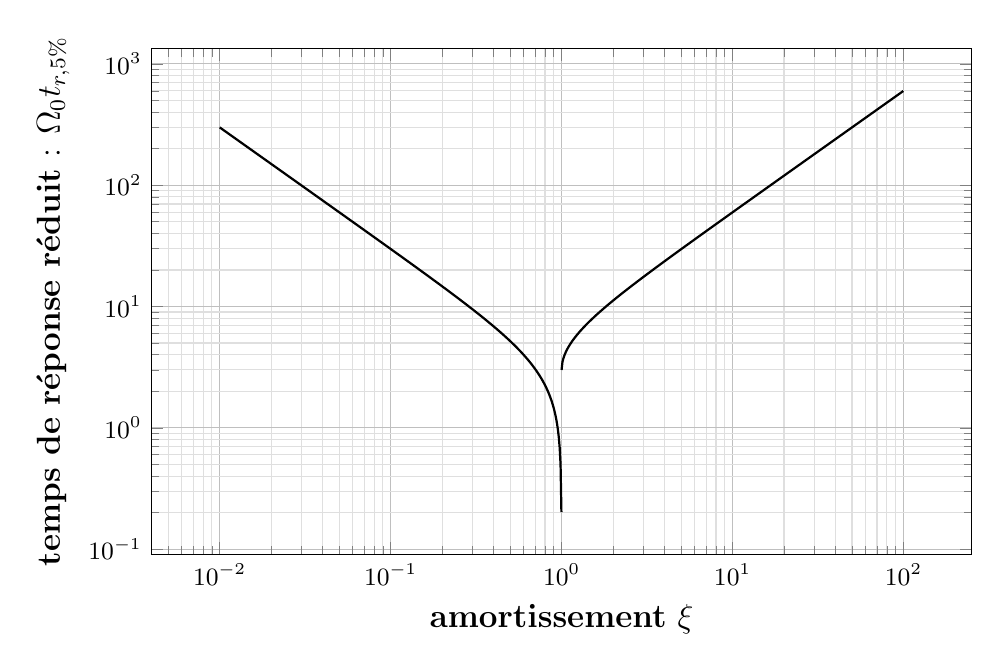
\begin{tikzpicture}
\begin{loglogaxis}[
    width=12cm,
    height=8cm,
    grid=both,
    minor grid style={gray!25},
    major grid style={gray!50},
    xlabel={\textbf{amortissement} $\xi$},
    ylabel={\textbf{temps de réponse réduit} : $\Omega_0 t_{r,5\%}$},
    xlabel style={font=\large},
    ylabel style={font=\large},
    tick label style={font=\small},
]

\addplot[
    thick,
    domain=0.01:0.999,
    samples=400,
]
{ -ln(0.05)*sqrt(1 - x^2)/x };

\addplot[
    thick,
    domain=1:100,
    samples=400,
]
{ -ln(0.05)*(x + sqrt(x^2 - 1)) };

\end{loglogaxis}
\end{tikzpicture}